\documentclass[a4paper,12pt]{article}
\usepackage{graphicx,amsmath,amssymb,listings,xcolor,tikz,caption,float}
\usepackage{hyperref}
\title{Development of an Arduino-Powered Digital Clock with Timer Capability}
\author{Arnav M - EE24BTECH11006}
\date{\today}

\begin{document}

\maketitle

\begin{abstract}
This document outlines the creation of an Arduino-controlled digital clock that integrates a timer function. The design utilizes a 7447 BCD-to-7-segment decoder in conjunction with common anode (active-low) 7-segment displays. User interaction is facilitated through push buttons, while precise timekeeping is achieved using a timer interrupt. Multiplexing is employed to efficiently manage six display digits representing hours, minutes, and seconds.
\end{abstract}

\section{Introduction}
Digital clocks serve as fundamental components in embedded systems. This project implements an Arduino-driven timekeeping device capable of displaying hours, minutes, and seconds, while also featuring a countdown timer mode. The design incorporates a 7447 decoder for efficient digit control and active-low common anode displays. The clock operates using a multiplexed display strategy and allows user adjustments via pushbutton inputs.

\section{System Components}
\subsection{Hardware Elements}
The system consists of the following hardware components:
\begin{itemize}
    \item \textbf{Arduino Microcontroller:} Responsible for time management, input processing, and controlling display operations.
    \item \textbf{7447 BCD-to-7-Segment Decoder:} Converts binary-coded decimal (BCD) input from the Arduino into signals to drive the 7-segment display.
    \item \textbf{Six Common Anode 7-Segment Displays:} Active-low displays used for showing the time in HH:MM:SS format.
    \item \textbf{Five Push Buttons:} Used to increment time, switch modes, and reset values.
    \item \textbf{Resistors:} Six $220\,\Omega$ resistors protect the displays by limiting current.
\end{itemize}

\subsection{Circuit Connections}
\subsubsection{Interfacing BCD with the 7447 Decoder}
The Arduino outputs BCD signals via digital pins PD2 through PD5, directing them to the 7447 decoder. As the displays are common anode, the decoder outputs operate in active-low mode. The wiring details are provided in Table~\ref{tab:decoder}.

\begin{table}[H]
    \centering
    \begin{tabular}{|c|c|}
        \hline
        \textbf{Arduino Pin} & \textbf{7447 BCD Input} \\
        \hline
        PD2 & A \\
        PD3 & B \\
        PD4 & C \\
        PD5 & D \\
        \hline
    \end{tabular}
    \caption{BCD Inputs to 7447 Decoder}
    \label{tab:decoder}
\end{table}

\begin{figure}[H]
\centering
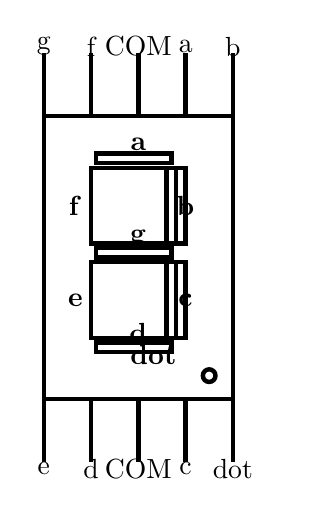
\begin{tikzpicture}[scale=0.4]
  [
    scale=1,
    >=stealth,
    point/.style = {draw, circle,  fill = black, inner sep = 0.5pt},
    dot/.style   = {draw, circle,  fill = black, inner sep = .2pt},
  ]

%Vertices of the main display rectangle
\def \xmin{0}
\def \xmax{6}
\def \ymin{0}
\def \ymax{-9}

%Number of pins on a side
\def \n{5}
\def \k{1.6}

%Draw the display rectangle
\draw[ultra thick] (\xmin,\ymin)rectangle (\xmax,\ymax);

%Define height of pins and their separation
\def \height{2}
\pgfmathsetmacro{\wid}{(\xmax-\xmin)/(\n-1)}

%Defining y axis divisions
\pgfmathsetmacro{\ywid}{(\ymin-\ymax)/(\n-2)}

\foreach \i in {0,...,4}
{
\draw[ultra thick] (\xmin + \i*\wid, \ymin) -- (\xmin + \i*\wid, \ymin + \height); 
\draw[ultra thick] (\xmin + \i*\wid, \ymax) -- (\xmin + \i*\wid, \ymax -\height); 
}
%%
%%%
\foreach [count=\i] \j in {g,f,COM,a,b}{
            \node (\i) at ( -1.5 + \i*\wid,\height+0.2) {\j} ;
            }
\foreach [count=\i] \j in {e,d,COM,c,dot}{
            \node (\i) at ( -1.5 + \i*\wid,\ymax -\height-0.2) {\j} ;
            }

\foreach [count=\i] \j in {\textbf{a},\textbf{g},\textbf{d}}
{            
\draw[ultra thick] (\xmin+1.1*\wid,{\ymin-(\i-0.5)*\ywid} ) rectangle +(\k*\wid,0.3 );
\node (\i) at ( \xmin + 2*\wid,{\ymin-(\i-0.7)*\ywid}) {\j} ;
}
\foreach [count=\i] \j in {\textbf{f},\textbf{e}}
{            
\draw[ultra thick] (\xmin+\wid,{\ymin-(\i+0.35)*\ywid} ) rectangle +(03,\k*\wid );
\node (\i) at ( \xmin + \wid-0.5,{\ymin-(\i-0.05)*\ywid}) {\j} ;
}
\foreach [count=\i] \j in {\textbf{b},\textbf{c}}
{            
\draw[ultra thick] (\xmin+2.6*\wid,{\ymin-(\i+0.35)*\ywid } ) rectangle +(0.3,\k*\wid );
\node (\i) at ( \xmin + 3*\wid,{\ymin-(\i-0.05)*\ywid}) {\j} ;
}

%
\draw[ultra thick] (\xmax - 0.5*\wid,{\ymax+0.25*\ywid}) circle [radius=0.2];
\draw[ultra thick](\xmax - 0.5*\wid,{\ymax+0.25*\ywid}) node[sloped, anchor=center, above, text width=2.0cm]{\textbf{dot}};    
\end{tikzpicture}
\caption{Interfacing Seven Segment Display with Arduino}
\label{fig:bcd_decoder}
\end{figure}

\subsubsection{Multiplexing Display Digits}
To efficiently control all six digits with a limited number of Arduino pins, a multiplexing approach is implemented. This technique allows the Arduino to activate each digit sequentially at high speed, creating the illusion of a continuously lit display. Table~\ref{tab:display_pins} summarizes the display pin connections.

\begin{table}[H]
    \centering
    \begin{tabular}{|c|c|}
        \hline
        \textbf{Digit Position} & \textbf{Arduino Pin} \\
        \hline
        Seconds (Units) & 6 \\
        Seconds (Tens)  & 7 \\
        Minutes (Units) & 8 \\
        Minutes (Tens)  & 9 \\
        Hours (Units)   & 10 \\
        Hours (Tens)    & 11 \\
        \hline
    \end{tabular}
    \caption{7-Segment Display Digit Selection Pins}
    \label{tab:display_pins}
\end{table}

\begin{figure}[H]
\centering
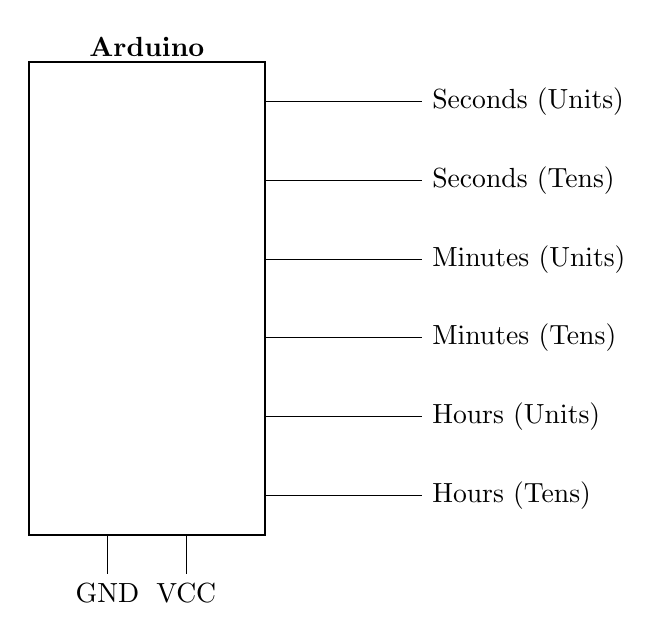
\begin{tikzpicture}
    % Draw Arduino
    \draw[thick] (0,0) rectangle (3,6);
    \node at (1.5, 6.2) {\textbf{Arduino}};
    
    % Digit lines
    \foreach \y/\pos in {5.5/6, 4.5/7, 3.5/8, 2.5/9, 1.5/10, 0.5/11} {
        \draw (3, \y) -- (5, \y);
    }
    
    % Displays
    \foreach \y/\pos in {5.5/Seconds (Units), 4.5/Seconds (Tens), 3.5/Minutes (Units), 2.5/Minutes (Tens), 1.5/Hours (Units), 0.5/Hours (Tens)} {
        \node[right] at (5, \y) {\pos};
    }
    
    % Ground and VCC
    \draw (1, 0) -- (1, -0.5) node[below] {GND};
    \draw (2, 0) -- (2, -0.5) node[below] {VCC};
\end{tikzpicture}
\caption{Multiplexing Display Digits with Arduino}
\label{fig:multiplexing}
\end{figure}

\section{Software Design and Implementation}
\subsection{System Operation}
The Arduino-based system operates in two modes:
\begin{itemize}
    \item \textbf{Clock Mode:} Displays hours, minutes, and seconds, incrementing the time every second.
    \item \textbf{Timer Mode:} Allows the user to set a countdown timer, decrementing the time until it reaches zero.
\end{itemize}
The system switches between these modes using a dedicated button. Upon completion of the countdown, the display blinks to indicate the end of the timer.

\subsection{Time Management Using Interrupts}
Timer interrupts ensure precise timekeeping. A 1ms tick is generated using \textbf{Timer0} configured in CTC (Clear Timer on Compare Match) mode. Time increments occur every 1000ms, and the system updates the display accordingly.

\subsection{User Interaction via Push Buttons}
Five push buttons provide user interaction:
\begin{itemize}
    \item \textbf{Increment Buttons:} Used to adjust hours, minutes, and seconds.
    \item \textbf{Mode Button:} Switches between clock and timer modes.
    \item \textbf{Pause/Resume Button:} Pauses and resumes the clock or timer.
    \item \textbf{Reset Button:} Long press resets the clock or timer values.
\end{itemize}

\subsection{Error Handling and Safety Measures}
Boundary conditions, such as exceeding 24 hours or 60 minutes, are automatically handled by resetting to zero. Button debouncing techniques prevent unintended multiple triggers.

\section{Conclusion}
This project successfully implements a digital clock with an integrated timer, leveraging a 7447 BCD decoder and multiplexed display control. Timer interrupts ensure precise timekeeping, and push buttons facilitate user interaction. The system efficiently switches between clock and timer modes while providing visual feedback through blinking when the timer completes. The project serves as an excellent demonstration of embedded system design principles.
The code is available in the following git hub link:
\url{https://github.com/arnavmahishi/EE1003/tree/main/hardware/clock}
\end{document}
.
